\chapter{Equitabilidad}\label{chap4}

	\section{Introducci\'on}

	La equitabilidad ha sido descrita de manera informal por Reshef et al. como la capacidad de una estadística para "asignar puntuaciones similares a relaciones igualmente ruidosas de diferentes tipos" \cite{Reshef2011}. Aunque útil, esta definición informal es imprecisa en el sentido de que no especifica lo que se entiende por "ruidoso" o "similar", y no especifica para qué relaciones debe cumplirse la propiedad mencionada.

	En su trabajo posterior  ''Equitability, interval estimation, and statistical power'', Reshef et al. (2015) \cite{Reshef2015}, se formaliz\'o la idea de Equitabilidad a travez del concepto del intervalo interpretativo, que funciona como estimaci\'on en intervalos de la cantidad de ruido presente en una relaci\'on de tipo desconocida. 

	En el contexto de este trabajo, nos interesa que las medidas de dependencia sean equitativas puesto que esto nos asegura que la medida de dependencia no est\'a sesgada hacia un tipo de relaci\'on en particular, y por lo tanto, nos ser\'a \'util para comprar comparar las distintas versi\'on de la transformac\'ion Box-Cox que definiremos en la secci\'on \ref{chap6}.

	En esta secci\'on se presentar\'a la definici\'on formal de equitabilidad, y de equitabilidad con respecto a $R^2$, recrearemos el experimento realizado por Reshef et al. (2016) \cite{Reshef2016} sobre la equitabilidad del $MIC_e$, y junto con esto se estudiar\'a la equitabilidad de las otras medidas propuestas en la Secci\'on \ref{chap4}. 

	\subsection[equidefiniciones]{Definiciones.}

	\subsection[equitabilidadmice]{Equitabilidad del $MIC_e$}

	Como se mencion\'o previamente, una de las principales motivaciones para la introducci\'on de $MIC$ fue la equidad, es decir, hasta qu\'e punto una medida de dependencia captura \'utilmente alguna noci\'on de la fuerza de una relaci\'on en un conjunto de relaciones est\'andar. En esto contexto en Reshef et al. (2016) \cite{Reshef2016} se realiz\~o un an\'alisis emp\'irico de la equidad de $MIC_e$ con respecto a R2 y su desempe\~no fue comparado con la correlaci\'on de distancia (Sz\'ekely et al., (2007)\cite{Szekely2007}; Sz\'ekely and Rizzo, (2009)\cite{Szekely2009}), la estimaci\'on de la informaci\'on mutua (Kraskov et al., 2004) y la estimaci\'on de la correlaci\'on m\'axima (Breiman and Friedman, 1985).

	Se comenz\'o evaluando la equidad en el conjunto de relaciones $Q$ definido anteriormente, un conjunto que ha sido analizado en otros trabajos previos (Reshef et al., 2011, 2015a; Kinney and Atwal, 2014). Los resultados, mostrados en la Figura \ref{reshef_2016_f3}, confirman la superior equidad del estimador $MIC_e$ en este conjunto de relaciones.

	Para evaluar la equidad de manera m\'as objetiva sin depender de un conjunto de funciones curado manualmente, se analizaron 160 funciones aleatorias extra\'idas de una distribuci\'on de proceso Gaussiano con un kernel de funci\'on radial con una de ocho posibles anchuras en el conjunto $\{0.01, 0.025, 0.05, 0.1, 0.2, 0.25, 0.5, 1\}$ para representar una variedad de complejidades de relaciones posibles. Los resultados, mostrados en la Figura \ref{reshef_2016_f4}, muestran que $MIC_e$ supera a los m\'etodos existentes en t\'erminos de equidad con respecto a $R^2$ en estas funciones tambi\'en. Tambi\'en se examin\'o el efecto de las relaciones at\'ipicas en los resultados al muestrear repetidamente subconjuntos aleatorios de 20 funciones de este gran conjunto de relaciones y medir la equidad de cada m\'etodo en promedio sobre los subconjuntos; los resultados fueron similares.

	Una caracter\'istica del desempe\~no de $MIC_e$ en estas relaciones elegidas al azar, como se muestra en la Figura \ref{reshef_2016_f4}, es que parece ser m\'inimamente sensible a la anchura del proceso Gaussiano del cual se extrae una relaci\'on dada. Esto contrasta, por ejemplo, con la estimaci\'on de la informaci\'on mutua, que muestra una sensibilidad pronunciada a este par\'ametro que le impide ser altamente equitativa cuando hay relaciones con diferentes anchuras en el mismo conjunto de datos.

	\begin{figure}[H] 
		\centering
		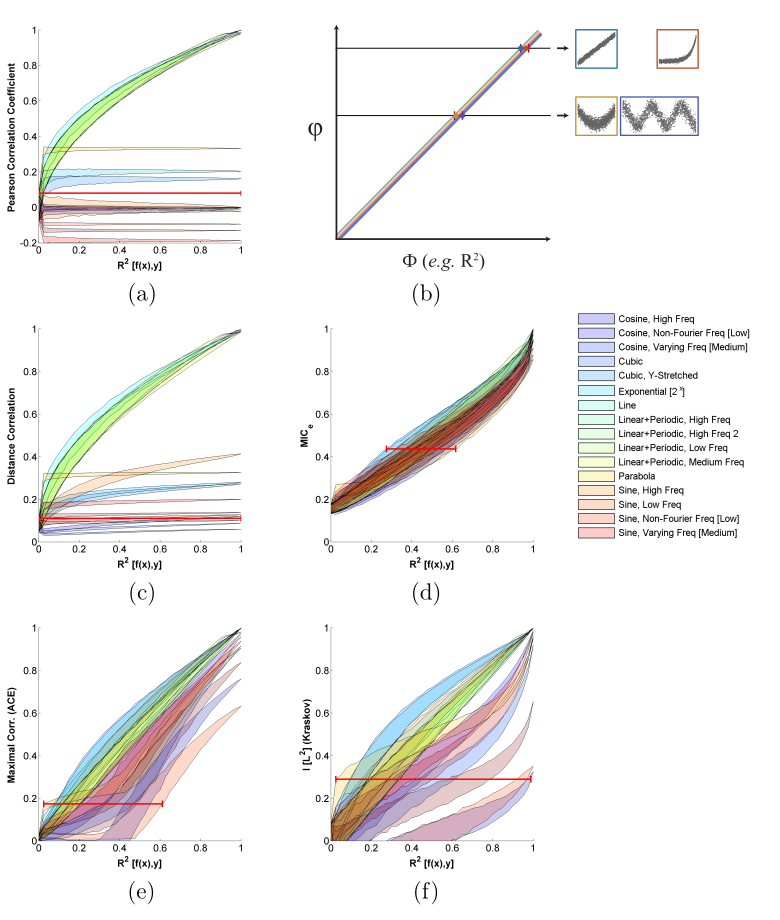
\includegraphics[scale = 0.4]{reshef_2016_fig3.png}
		\caption{Equitabilidad con respecto a $R^2$ en un conjunto de relaciones funcionales ruidosas de $(a)$ el coeficiente de correlaci\~on de Pearson, $(b)$ una medida hipot\~etica de dependencia $\varphi$ con equitabilidad perfecta, $(c)$ la correlaci\~on de distancia, $(d)$ $\mathrm{MIC}_e$, $(e)$ estimaci\~on de correlaci\~on m\~axima y $(f)$ estimaci\~on de informaci\~on mutua. Para cada relaci\~on, una regi\~on sombreada denota los valores estimados en el percentil 5 y 95 de la distribuci\~on muestral de la estad\~istica en cuesti\~on en esa relaci\~on en cada valor de $R^2$. El gr\~afico resultante muestra qu\~e valores de $R^2$ corresponden a un valor dado de cada estad\~istica. El intervalo rojo en cada gr\~afico indica el rango m\~as amplio de valores de $R^2$ que corresponden a un valor de la estad\~istica; cuanto m\~as estrecho sea el intervalo rojo, mayor ser\~a la equitabilidad. Un intervalo rojo con ancho 0, como en $(b)$, significa que la estad\~istica refleja solo $R^2$ sin depender del tipo de relaci\~on, como se demuestra en los pares de miniaturas de relaciones de diferentes tipos con valores id\~enticos de $R^2$.}
		\label{reshef_2016_f3}
	\end{figure}

	\begin{figure}[H] 
		\centering
		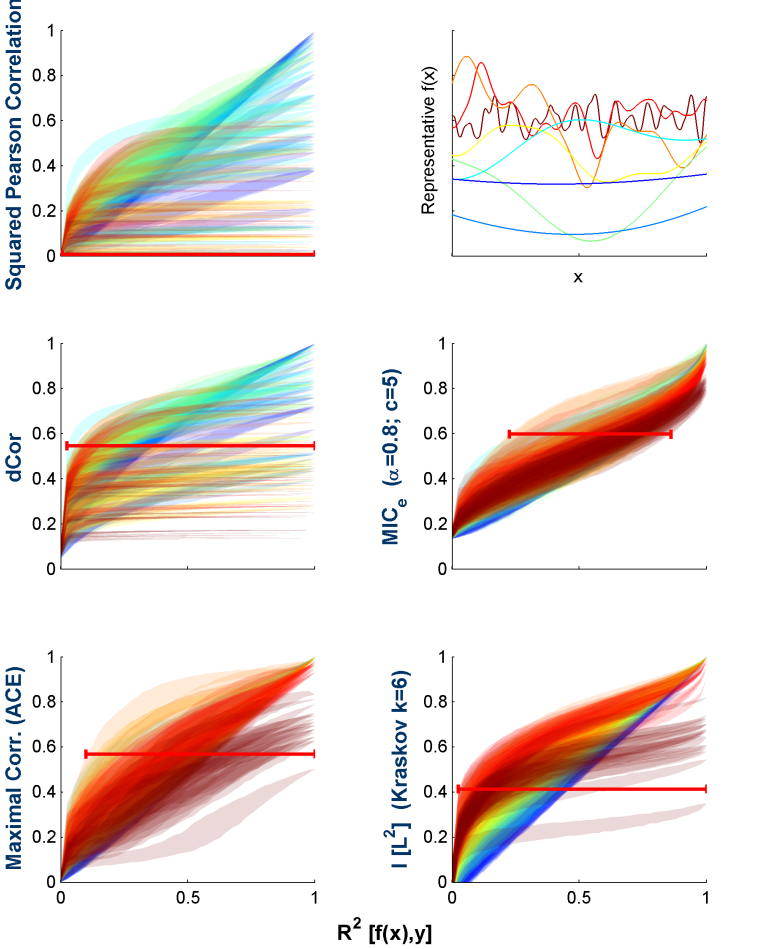
\includegraphics[scale = 0.4]{reshef_2016_fig4.png}
		\caption{Equitabilidad de los m\~etodos examinados en funciones extra\~idas al azar de una distribuci\~on de proceso gaussiano. Cada m\~etodo se eval\~ua como se muestra en la Figura \ref{reshef_2016_f3}, con un intervalo rojo que indica el rango m\~as amplio de valores de $R^2$ correspondiente a cualquier valor de la estad\~istica; cuanto m\~as estrecho sea el intervalo rojo, mayor ser\~a la equitabilidad. Cada regi\~on sombreada corresponde a una relaci\~on, y las regiones est\~an coloreadas seg\~un el ancho de banda del proceso gaussiano del que se muestrearon. Las relaciones de muestra para cada ancho de banda se muestran en la esquina superior derecha con colores correspondientes.}
		\label{reshef_2016_f4}
	\end{figure}